\chapter[High brightness ion beam through MOC]{High brightness ion beam through magneto-optical compression\label{ch:newsource}}
%\documentclass [10pt,a4paper] {article}
%\documentclass[aip,jap,twocolumn,preprint,showpacs]{revtex4}
%\documentclass[aip,jap,reprint,twocolumn,showpacs,floatfix]{revtex4-1}
%\documentclass[]{iopart}
%
%\usepackage{graphicx}% Include figure files
%\usepackage{dcolumn}% Align table columns on decimal point1
%\usepackage{bm}% bold math
%\usepackage[caption=false]{subfig}
%%\usepackage{subfigure}  % use for side-by-side figures
%
%% to solve conflict between ansmath and iopart
%\expandafter\let\csname equation*\endcsname\relax						
%\expandafter\let\csname endequation*\endcsname\relax
%
%\usepackage{amsmath}	% split equations in more lines
%%\usepackage[OPTIONS]{preview}
%
%\begin{document}

%\title{High brightness ion beam through magneto-optical compression}
%
%\author{N Debernardi, R P M J W Notermans, D J N Kusters, S B van der Geer, P H A Mutsaers, O J Luiten and E J D Vredenbregt}
%\address{Department of Applied Physics, Eindhoven University of Technology, P.O Box 513, 5600 MB Eindhoven, the Netherlands}
%\ead{E.J.D.Vredenbregt@tue.nl}
%
%\date{\today{}}

\begin{abstract}
We show that the combination of a high flux atomic beam originating from a Knudsen cell and the technique of magneto-optical compression, can be used to create an extremely bright ion beam with a low longitudinal energy spread. Realistic simulations of laser cooling and ion beam formation are reported, taking into account the effect of disorder-induced heating. This research shows that a reduced brightness on the order of $10^7$~A/m$^2$~sr~eV with an ion current of tens of pA and an energy spread of about 1 eV can be achieved with a $^{87}$Rb$^+$ beam. This is possible when the so called pencil-beam regime is reached, where the beam size is smaller than the transverse inter-particle spacing.
\footnote{The work described in this chapter by \underline{N. Debernardi}, R P M J W Notermans, D J N Kusters, S B van der Geer, P H A Mutsaers, O J Luiten and E J D Vredenbregt has been submitted for publication to New J. Phys.}
\end{abstract}

\clearpage

\section{Introduction}
Focused Ion Beams (FIBs) are widely used in the semiconductor industry. The properties of the ion source that is implemented in the FIB ultimately limit the characteristics of the beam. The current state-of-art is the Liquid-Metal Ion Source (LMIS), which has a longitudinal energy spread of 4.5 eV and a reduced brightness of $10^6$~A/m$^2$~sr~eV \cite{Orloff_RoSI_93}. The minimum spot size that can be achieved with a LMIS is limited by the chromatic aberration due to the relatively large longitudinal energy spread of the source. Alternative sources, that combine a lower energy spread with a comparable or even a higher brightness, are needed to enable further development of FIBs to keep up with the trend of the production of smaller and smaller semiconductor components \cite{Moore_E_65}.

In previous work \cite{Debernardi2012, Reijnders_PRL_09}, the properties of an ion beam extracted from an ultracold ion source (UCIS) have been investigated. $^{85}$Rb atoms were collected, cooled down in a magneto-optical trap (MOT), and subsequently photo-ionized. In this way, ion bunches are extracted and accelerated with a high repetition rate. An upper limit for the reduced brightness was set at $8 \times 10^4$~A/m$^2$~sr~eV, but simulations showed that disorder-induced heating does reduce the brightness by one to two orders of magnitude, depending on the extracted current. The brightness of a MOT-based source therefore remains far below that of the LMIS. The strength of the UCIS, and of similar sources as the MOTIS \cite{Hanssen_PRA_06, Hanssen_NL_08}, is in its versatility, since several different atomic species can be used \cite{Steele_JVSTB_10}. Moreover, energy spread down to 20 meV has been demonstrated \cite{Reijnders_PRL_09}, substantially lower than a LMIS.

In this paper, a new source concept with better performance with respect to the UCIS is investigated. The essential difference with the UCIS is that this new source is based on two-dimensional magneto-optical compression of an atomic beam rather than three-dimensional magneto-optical trapping of an atomic vapor. Extending the original idea of Freinkman \textit{et al.} \cite{Freinkman2004}, an atomic beam laser-cooled ion source (ABLIS) is proposed, as schematically shown in figure \ref{fig:setup_newsource}.
\begin{figure}[tbh!]
    \centering
        \includegraphics[width=0.6\linewidth]{pics/newsource/setup4}
    \caption{Schematic drawing of the setup in the $xz$ plane, not to scale. From the left to the right hand side, an atomic beam $B$, formed from an aperture $S$ of a Knudsen cell $K$, is skimmed by an aperture with area $A_i$. In the MOC, the beam is cooled with 2 pairs (in the drawing only one pair is shown) of counter-propagating laser beams perpendicular to the z-axis (with $\sigma^+$ and $\sigma^-$ polarization) and, at the same time, it is compressed with a magnetic gradient $G$ into an aperture with area $A_f$. The quantities $d$ and $d_f$ represents either the aperture radius (for the analytical model) or the half-width aperture size (for the simulations). The distance between $A_i$ and $A_f$ is $L$. The aperture $A_f$ is put at a positive potential. Finally, the beam is ionized and an ultracold ion beam $U$ is created. The ionization process occurs in an electric field so that the beam is also accelerated toward the last aperture $H$ which is grounded.} 
    \label{fig:setup_newsource}
\end{figure}
The setup can be divided in three parts: in the first part, an atomic beam $B$ is formed by skimming with an aperture of area $A_i$ the expansion of a gas or vapor emanating from a Knudsen cell with an aperture of area $S$. In the second part, the beam is cooled down transversally by two pairs of counter-propagating laser beams and simultaneously compressed in the presence of a magnetic field gradient. This component is named MOC (Magneto-Optical Compressor). In the third part, after passing through a second aperture with area $A_f$, the atomic beam is crossed with an ionization laser beam in an electric field and an ultracold ion beam $U$ is then created. The second aperture is put at a positive potential and the anode $H$ is grounded, so that the electric field $\vec{E}$ accelerates the ions toward $H$. The quantities $d$ and $d_f$ represent either the aperture radius (for the analytical model) or the half-width aperture size (for the simulations). 

Very large gains in atomic beam brightness have been obtained with laser cooling methods in the past \cite{Tempelaars2002, Lison1999}. However, this required extensive beam lines that are impractical for mounting on a FIB column. Here we investigate what brightness a compact setup involving only a source and short compressor can deliver. The ABLIS exploits a high atomic flux that effuses from a Knudsen cell and converts, cools and compresses it into a micrometer range transverse beam size with milliKelvin transverse temperature, greatly increasing its brightness. By restricting the diameter of the atomic beam with aperture $A_f$, before the atoms are converted to ions, the so-called ``pencil-beam'' regime \cite{Tiemeijer1999} can be reached: space charge forces in the transverse direction are negligible and the brightness should be less influenced by disorder-induced heating.

This paper first presents an analytical model which can be used to predict the general dependence of the source performance on some key variables. The reduced brightness and the current are examples of the source properties that will be calculated. Secondly, this model is used for a preliminary optimization and as a starting point for particle tracing simulations, which are required in order to include a more realistic physics and to avoid limitations of the model. Several simulations of the intensification of the atomic beam MOC are calculated with the computer code COOL~\cite{Vredenbregt_AJoP_03}, which treats Doppler cooling \cite{Metcalf_Book_99} of individual atoms in magnetic fields. The best case scenario is then used as input for simulations of the ion beam formation using the General Particle Tracer code (GPT) \cite{gpt}, which treats the motion of ions in external electromagnetic fields where the Coulomb interaction between ions is taken into account. Finally, it is shown that, according to the simulations, this source can achieve both a higher brightness and a lower energy spread than LMIS, at the same time.

\section{Analytical model of the source}\label{sec:anamodel}
An analytical model is developed in order to estimate the performance of the source and to have a starting point for the optimization in the parameter space of several variables, before performing simulations. The  model is based on a standard theoretical treatment of laser cooling, such as formulated by Metcalf and Van der Straten \cite{Metcalf_Book_99}.

The flux $\Phi_i$ of atoms emanating from a Knudsen cell with an aperture of area $S$ within a small azimuthal angle $\theta$ and at an atomic density $n$ is given by 
\begin{equation}
    \Phi_i = \frac{1}{4} n S \left\langle v \right\rangle \theta^2.
    \label{eq:flux_i}
\end{equation}
The density $n=p/(k_b T_s)$ of the atoms can be controlled with the temperature $T_s$ of the Knudsen cell, where $k_b = 1.381 \times 10^{-23}$ m$^2$ kg s$^{-2}$ K$^{-1}$ is Boltzmann's constant. For alkali metal vapors above the melting temperature, we can approximate the pressure as $p=p^*\exp(-T^*/T_s)$ \cite{Haynes_Book_12}, where the constants $p^*$ and $T^*$ depend on the atomic element, the physical state and the source temperature, and they can be calculated from reference \cite{Haynes_Book_12}. Table \ref{tab:Rb_atomic_consts} lists the atomic properties of rubidium, which is the atomic species used in this paper.
\begin{table}[h!]
	\centering
	\caption{Atomic constants used in the calculations and the simulations. Note that the values of $p^*$ and $T^*$ are valid for a set of source temperatures ranging from $312$~K (melting point) to $550$~K \cite{Haynes_Book_12}.}
	\begin{center}
		\begin{tabular}{|l|l|l|l|} \hline
		{Parameter (unit)} & {Symbol} & {$^{85}$Rb} & {$^{87}$Rb} \\ \hline
		{Mass (amu)} \cite{Haynes_Book_12_b}& $m$ & {84.91 } & {86.91 } \\ 
		{Pressure constant (Pa)} \cite{Haynes_Book_12}& $p^*$ & {$2.08 \times 10^9$ } & {$2.08  \times 10^9$ } \\ 
		{Temperature constant (K)} \cite{Haynes_Book_12}& $T^*$ & {$9.30 \times 10^3$ }	& {$9.30 \times 10^3$ } \\ 
		{Natural linewidth (MHz)} \cite{Metcalf_Book_99}& $\Gamma/2 \pi$ & {5.98 } & {5.98 }	\\ 
		{Saturation intensity (W/m$^2$)} \cite{Metcalf_Book_99}& $I_s$ & {16.4} & {16.4} \\
		{Abundance (\%)} \cite{Haynes_Book_12_b} & {$ab$} & {72.2} & {27.8}	\\  
		{Cooling wavelength (nm)} \cite{Metcalf_Book_99}& {$\lambda$} & {780} & {780} \\
		{Nuclear spin quantum number} \cite{Haynes_Book_12_b}& $I$ & {$5/2$ } & {$3/2$ }	\\ \hline
		\end{tabular}
	\end{center}
	\label{tab:Rb_atomic_consts}
\end{table}

The longitudinal velocity $v_z$ follows a Maxwell-Boltzmann distribution and its average $\left\langle v \right\rangle$ is related to the source temperature as
\begin{equation}
    \left\langle v \right\rangle = \sqrt{\frac{8 k_b T_s}{\pi m}},
    \label{eq:t_thermal}
\end{equation}
where $m$ is the mass of the atom. \\
The angle is defined as $\theta=d/l$ where $d$ is the aperture size (intended as aperture radius in this analytical model) and $l$ is the expansion stage length between the Knudsen cell and the MOC, as shown in figure \ref{fig:setup_newsource}.\\ 
The flux of equation (\ref{eq:flux_i}) corresponds to a reduced initial brightness $B_r^i$, which can be calculated as \cite{Luiten_IJoMPA_07}
\begin{equation}
    B_r^i = \frac{e J}{\pi k_b T'_s}= \frac{e^2 \Phi_i / S}{\pi k_b T_s \theta^2},
    \label{eq:br_i}
\end{equation}
where $e = 1.602 \times 10^{-19}$~C is the elementary charge and $T'_s=T_s \theta^2$ is the effective source temperature, due to the presence of the initial aperture $A_i$. This is not the brightness of the atomic beam, but an equivalent brightness for an ion beam with the same properties. The extra $e$ factor in the previous equation is necessary to convert the resulting reduced brightness in unit of A/m$^2$~sr~eV. In what follows, the apertures $S$ and $A_i$ are set to be the same size as a simplification in this model.\\

In the second stage, the beam brightness can be increased with the use of a magneto-optical compressor stage. The forces in a MOC are two-dimensional, but we are going to treat the two transverse dimensions as independent, assuming that the total force on an atom can be written as the sum of the radiation pressure of the separate laser beams. Then the problem is quasi-2D. Laser cooling is asserted with two pairs of laser beams, where each pair is made up of two counter propagating laser beams with respectively a $\sigma^+$ and a $\sigma^-$ polarization. Moreover, we consider a transition between two levels with angular momentum quantum numbers $F=0$ and $F=1$. The fact that rubidium has more than one ground state due to hyperfine splitting is ignored, i.e. we assume the presence of a sufficiently strong re-pump laser beam in the experiment. The re-pump laser beam is necessary since the time spent by an atom for traveling in the MOC is about 4 times longer than the average decay time to the wrong ground state. This is calculated using the values shown in table \ref{tab:parametervalues_ana} and the scattering rate formula found in \cite{Metcalf_Book_99}.
\begin{table}[h!]
	\centering
	\caption{Parameter values for a 2-level $^{85}$Rb atom used in the analytical model and the simulation.}
	\begin{center}
		\begin{tabular}{|l|l|l|} \hline
		{Parameter (unit)} & {Symbol} & {Analytical model} \\ \hline
		{Expansion length (m)} & $l$ & {$3.9 \times 10^{-2}$} 	\\ 
		{Initial aperture size (m)} & $d$ & {$3.1 \times 10^{-4}$} 	\\ 
		{Source temperature (K)} & $T_s$ & {$350$} 	\\ 
		{Cooling and compression length (m)} & $L$ & {$5 \times 10^{-2}$} 	\\ 
		{Saturation parameter (-)} & $s_0$ & {$2$} 	\\ 
		{Detuning ($\Gamma$)} & $\delta$ & {$-0.5$} 	\\
		{Magnetic gradient (T/m)} & $G$ & {$1$}	\\ \hline
		\end{tabular}
	\end{center}
	\label{tab:parametervalues_ana}
\end{table}

For one set of counter propagating beams, the force $F_{MOC}$ acting on an atom has the expression \cite{Metcalf_Book_99}
\begin{equation}
    %F = \frac{\hbar k s_0 \Gamma/2}{1 + s_0 + \left( \frac{2 \delta_{eff}}{\Gamma} \right)^2},
    F_{MOC} = \hbar k s_0 \Gamma/2 \left[ \left[1 + s_0 + 4 \left( \delta_{eff}^+ \right)^2 \right]^{-1} - \left[1 + s_0 + 4 \left( \delta_{eff}^- \right)^2 \right]^{-1} \right].
    \label{eq:force_newsource}
\end{equation}
In this equation, $s_0 = I_L/I_s$ is the saturation parameter, with $I_L$ as the laser beam intensity, $I_s$ as the saturation intensity and $\Gamma$ as the natural linewidth of the atomic transition. Moreover, $\delta_{eff}^{\pm}$ is the effective detuning of the laser beam, which is the sum of three terms:
\begin{equation}
    %\delta_{eff}^{\pm} = \delta \pm k v_x \pm \frac{G \mu_b x}{\hbar},
    \delta_{eff}^{\pm} = \delta_n \pm \frac{k v_x}{\Gamma} \pm \frac{G \mu_b x}{\Gamma \hbar},
    \label{eq:detu_eff}
\end{equation}
where $\delta_n=\delta/\Gamma$ is the normalized laser detuning with $\delta$ as the laser detuning in unit of $\Gamma$, $k=2 \pi / \lambda$ is the wave number, $\lambda$ is the laser wavelength, $v_x$ is the transverse velocity of the atom, $G$ is the magnetic field gradient, $\mu_b = 9.27 \times 10^{-24}$~J/T is the Bohr magneton, $x$ is the transversal position of the atom and finally $\hbar = 1.055 \times 10^{-34}$~J~s is Dirac's constant. In equation (\ref{eq:detu_eff}), the positive sign of $\delta_{eff}$ is for a laser beam traveling along the positive $x$-axis direction and the negative one is for a laser beam traveling in the opposite direction.
The force of equation (\ref{eq:force_newsource}) accelerates an atom according to Newton's second law $F_{MOC}=m a$.

The Doppler temperature $T_D$, defined as \cite{Foot_Book_05} 
\begin{equation}
    %T_D = \hbar \Gamma / 2 k_b,
    %T_D = - \frac{\hbar \Gamma}{4 k_B} \Big( \frac{\Gamma}{2\delta}(1 + s_0) + \frac{2 \delta}{\Gamma}\Big),
    T_D = - \frac{\hbar \Gamma}{4 k_b} \Big( \frac{1 + s_0}{2\delta_n} + 2 \delta_n \Big),
    \label{eq:Tdoppler}
\end{equation}
is the minimum temperature reachable with elementary Doppler laser cooling. In order to efficiently cool to the Doppler temperature the atoms passing the first aperture $A_i$, the skimming aperture is sized to transit only atoms whose transverse velocity with respect to the atomic beam axis is smaller than the capture velocity $v_c = -\delta / k$~\cite{Metcalf_Book_99}. In what follows we will keep the maximum transverse velocity at a fixed value of $v_{max}=\Gamma/{2 k}$ which results in a opening angle of $\theta=v_{max}/\left\langle v \right\rangle=8$~mrad, i.e. the nominal value for a detuning of $-\Gamma/2$ (which is the optimum for laser-cooling \cite{Metcalf_Book_99}) and a source temperature of 350~K. This ensures that the transverse velocities of the atoms remain well within the capture range over most of the parameter range that we consider. For larger detunings, the brightness we obtain in this way probably then represents a lower limit that may be further increased by relaxing the criterion. After cooling, the brightness of the atomic beam $B_c$ becomes
\begin{equation}
    B_r^c = B_r^i \frac{T_s~{\theta}^2}{T_D} = \frac{e^2 \Phi / S}{\pi k_b T_D}.
    \label{eq:b_c}
\end{equation}
Using the values of table \ref{tab:parametervalues_ana}, the gain in brightness $T_s~\theta^2/T_D \approx 77$ only due to Doppler cooling is already very large.

With magneto-optical compression, in addition, the beam's area can be reduced, leading to an extra increase in the brightness. Using a compression length $L$ and a corresponding compression time $t$ defined as 
\begin{equation}
    t=L / \left\langle v \right\rangle,
    \label{eq:time}
\end{equation}
atoms from within an area $A_i=\pi d^2$ can be forced into a smaller area $A_f$. The initial aperture size $d$ is calculated with the values shown in table \ref{tab:parametervalues_ana} as \cite{Foot_Book_05}
\begin{equation}
    %d=\frac{a_{max} t^2}{4} = \frac{F L^2}{4 m \left\langle v \right\rangle^2} = 309 \times 10^{-6}~m.
    d=\frac{a_{max} L^2} {4 \left\langle v \right\rangle^2} = 3.1 \times 10^{-4}~\textrm{m},
    \label{eq:init_r}
\end{equation}
where the maximal acceleration is defined as $a_{max}=\lim_{(v_x~\to~v_c,~x~\to~0)}~F_{MOC}/m$.

The initial expansion stage length $l$ is calculated as
\begin{equation}
    l = \frac{d}{\theta} = 3.9 \times 10^{-2}~\textrm{m}.
    \label{eq:init_d}
\end{equation}

The final beam area is calculated assuming that atoms have reached equilibrium as $A_f=\pi k_b T_D/\kappa$. The spring constant $\kappa$ of the previous equation is given by
\begin{equation}
    \kappa = \lim_{v_x \to 0, x \to 0} \Big[ -\frac{\partial F_{MOC}}{\partial x} \Big] = -8 \mu_B G s_0 k \frac{\delta_n}{(1 + s_0 + 4 \delta_n^2)^2}.
    %\kappa = \mu_b G s_0 k,
    \label{eq:spring}
\end{equation}

After the compression the resulting reduced brightness of the atomic beam $B_r^f$ is then expressed as 
\begin{equation}
    B_r^f = B_r^c  \frac{A_i}{A_f} = \frac{e^2 \Phi / S}{\pi k_b T_D} \frac{A_i}{A_f}.
    \label{eq:br}
\end{equation}
We can now calculate the gain in brightness due to compression. From equation (\ref{eq:br}) and substituting the values of table \ref{tab:parametervalues_ana}, it results that $A_i/A_f=d^2 \kappa/k_b T_D \approx 900$. So compressing the beam (i.e. going beyond the ideas of Freinkmann \textit{et al} \cite{Freinkman2004}) gives a very large gain in brightness. The total gain in brightness due to cooling and compressing by using a MOC could result in about $7 \times 10^4$. 
More information on cooling and compressing of atoms can be found in \cite{Metcalf_Book_99, Foot_Book_05}.\\

An analytical solution for the reduced brightness $B_r^{ana}$ can be expressed as
\begin{equation}
\begin{split}
    B_r^{ana} =& -\left[ \frac{e^2 \mu_b \sqrt2~\pi^{5/2}}{k_b^{7/2}} \right] \cdot \left[ \frac{p^* \Gamma^2 \sqrt{m}}{\lambda} \right]\\ 
    &\cdot \left[\frac{G~L^4~s_0^3~\delta_n^7~\exp(-T^*/T_s)}{T_s^{7/2} (1+s_0)^2 (1+s_0+4~\delta_n^2)^4 (1+s_0+16~\delta_n^2)^2} \right].
    \label{eq:ana}
\end{split}
\end{equation}
%Eq. (\ref{eq:ana}) can be further rearranged into
%\begin{align}
%    B_r^{ana} = - \frac{16}{\sqrt{2 \pi^3}} \frac{e^2 \mu_B G s_0 A_i \Delta \theta^2}{\lambda \sqrt{m k_b^5}} \frac{p_0 \exp[-T_0/T_s]}{T_D^2 \sqrt{T_s}} \frac{\delta_n}{(1 + s_0 + 4\delta_n^2)^2}.
%    \label{eq:ana2}
%\end{align}
Equation (\ref{eq:ana}) is made up of three main factors included in square brackets: the first term includes all the numerical and physical constants together; the second term contains the constants which depend on the used atom; the last term contains all the parameters of the model over which we have external control. Equation (\ref{eq:ana}) is useful to see the dependence of the reduced brightness versus the parameters of the model ($L$, $G$, $s_0$, $\delta_n$ and $T_s$). Simulations will explore those parameters more in depth in section \ref{sec:results}.

In order to have a realistic starting point for simulations, we need to choose some values of the parameters since the dependence on $G$, $L$ and $T_s$, does not lead to an optimum for the reduced brightness. The brightness scales linearly with the magnetic gradient field. A magnetic gradient $G = 1$~T/m is chosen such that the spatial capture range is approximately equal to the radius of the aperture. The compression length is really important, since the brightness scales as $L^4$. The compression length is chosen to be 0.05~m in order to keep the setup compact and because that is the maximum size of ordinary optics elements. The source temperature can be increased as long as the mean free path $\Lambda$ of the particles is much larger than the aperture size of the Knudsen cell $d$. The mean free path of a particle is defined as \cite{Blundell_Book_06}
\begin{equation}
    \Lambda = \frac{k_b T_s}{\sqrt2 \pi p (2 r_{vdW})^2},
    \label{eq:mfp}
\end{equation}
where $r_{vdW} = 0.3$~nm is the typical Van der Waals radius for rubidium \cite{Mantina2009}. The quantity $\Lambda$ equals 0.5~m for $T_s=350$~K and it drops rapidly to 21~mm for $T_s=400$~K. A higher source temperature means a higher initial flux, but on the other hand, also the longitudinal velocity increases and this influences the efficiency of the compressor stage.
 
Figure \ref{fig:density} displays the reduced brightness of equation (\ref{eq:ana}) versus the saturation parameter and the normalized detuning in case of a 2-level $^{85}$Rb. For this calculation, the used parameters are summarized in table \ref{tab:parametervalues_ana} (except for the quantities $s_0$ and $\delta_n$ which are varied). Here there is a clear optimum, the maximum of the reduced brightness $B_r^{ana} = 2.1 \times 10^7$~A/m$^2$~sr~eV occurs at $\delta_n = -0.8$ (where $\kappa$ is maximized), and at $s_0 = 2$. From this plot, it is also interesting to note that increasing the laser intensity does not increase the brightness for $s_0 > 2$.
\begin{figure}[tbh!]
    \centering
        \includegraphics[width=0.7\linewidth]{pics/newsource/density}
    \caption{The analytical reduced brightness $B_r^{ana}$, in unit of A/m$^2$~sr~eV, plotted versus the saturation parameter and the normalized detuning in case of a 2-level $^{85}$Rb. The used parameters are shown in table \ref{tab:parametervalues_ana}, except from the quantities $s_0$ and $\delta_n$ which are varied.} 
    \label{fig:density}
\end{figure}


\section{Simulation and analysis} \label{sec:simu}
The result of the analytical model is used as a starting point for the simulations. The analytical model considered an ideal 2-level $^{85}$Rb whereas simulations use a realistic atom.

The simulation is made up of two parts. The program COOL \cite{Vredenbregt_AJoP_03} simulates the laser cooling and compression of the atomic beam effused from a Knudsen cell. The simulation is based on absorption and emission of individual photons, but a re-emitted photon does not interact anymore and it is basically "lost"; in other words, the simulation does not include optical thickness of the media into account. The code is unchanged compared to the version from reference \cite{Vredenbregt_AJoP_03} except for replacing the initial particle distribution with something more appropriate to our geometry, see section \ref{sec:initdistr}. The aperture sizes $d$ and $d_f$ in the simulation are meant as half-width aperture size, since square apertures are here used. The square aperture is chosen instead of a circular one because it is computationally simpler.

Finally, the ion tracing simulations are performed with the General Particle Tracer code (GPT) \cite{gpt}, where space charge forces are fully taken into account.

To summarize our computations in terms of the $z$ coordinate of the beam: a geometrical flux calculation is used for $0<z<l$ (see equation \ref{eq:initflux}), the COOL code is used for $l<z<l+L$ and the GPT code for $z>l+L$.

\subsection{Initial particle distribution} \label{sec:initdistr}
In COOL, the initial velocities and angles of the particles are initialized at the first aperture $A_i$ with a Monte Carlo algorithm, according to an appropriate geometrical boundary condition and the Maxwell-Boltzmann velocity distribution. The spatial distribution at the aperture is uniform since $d \ll l$. We approximate the situation by considering motion in the two transverse dimensions separately. For an initial longitudinal velocity, two simulations are performed, one for the $x$-direction and another one for the $y$-direction.

The longitudinal velocities follow the Maxwell-Boltzmann distribution \cite{Scoles1988}
\begin{equation}
  	f_v(v_z) d v_z = N \sqrt{\frac{2}{\pi}} \frac{v_z^2}{v_{\sigma}^3} \exp \Bigg[ - \frac{1}{2} \Big( \frac{v_z}{v_{\sigma}}\Big)^2  \Bigg] d v_z,   
  	\label{eq:initdistr_vel}
\end{equation}
where $v_{\sigma} = \sqrt{k_b T_s / m}$ is the thermal velocity of the atoms. The longitudinal velocity distribution is normalized to $N$, which is the total number of particles in the simulation. Figure \ref{fig:v_distr} shows an example of a typical velocity distribution obtained with $N=5 \times 10^5$ $^{87}$Rb particles effused at $T_s=400$ K. The distribution is fitted with equation (\ref{eq:initdistr_vel}). The thermal velocity determined from the fit is $(194.7 \pm 0.2)$ m/s and is in good agreement with the calculated value $v_{\sigma} =195$ m/s. %From this we conclude that the number of particles is large enough.
\begin{figure}[tbh!]
    \centering
        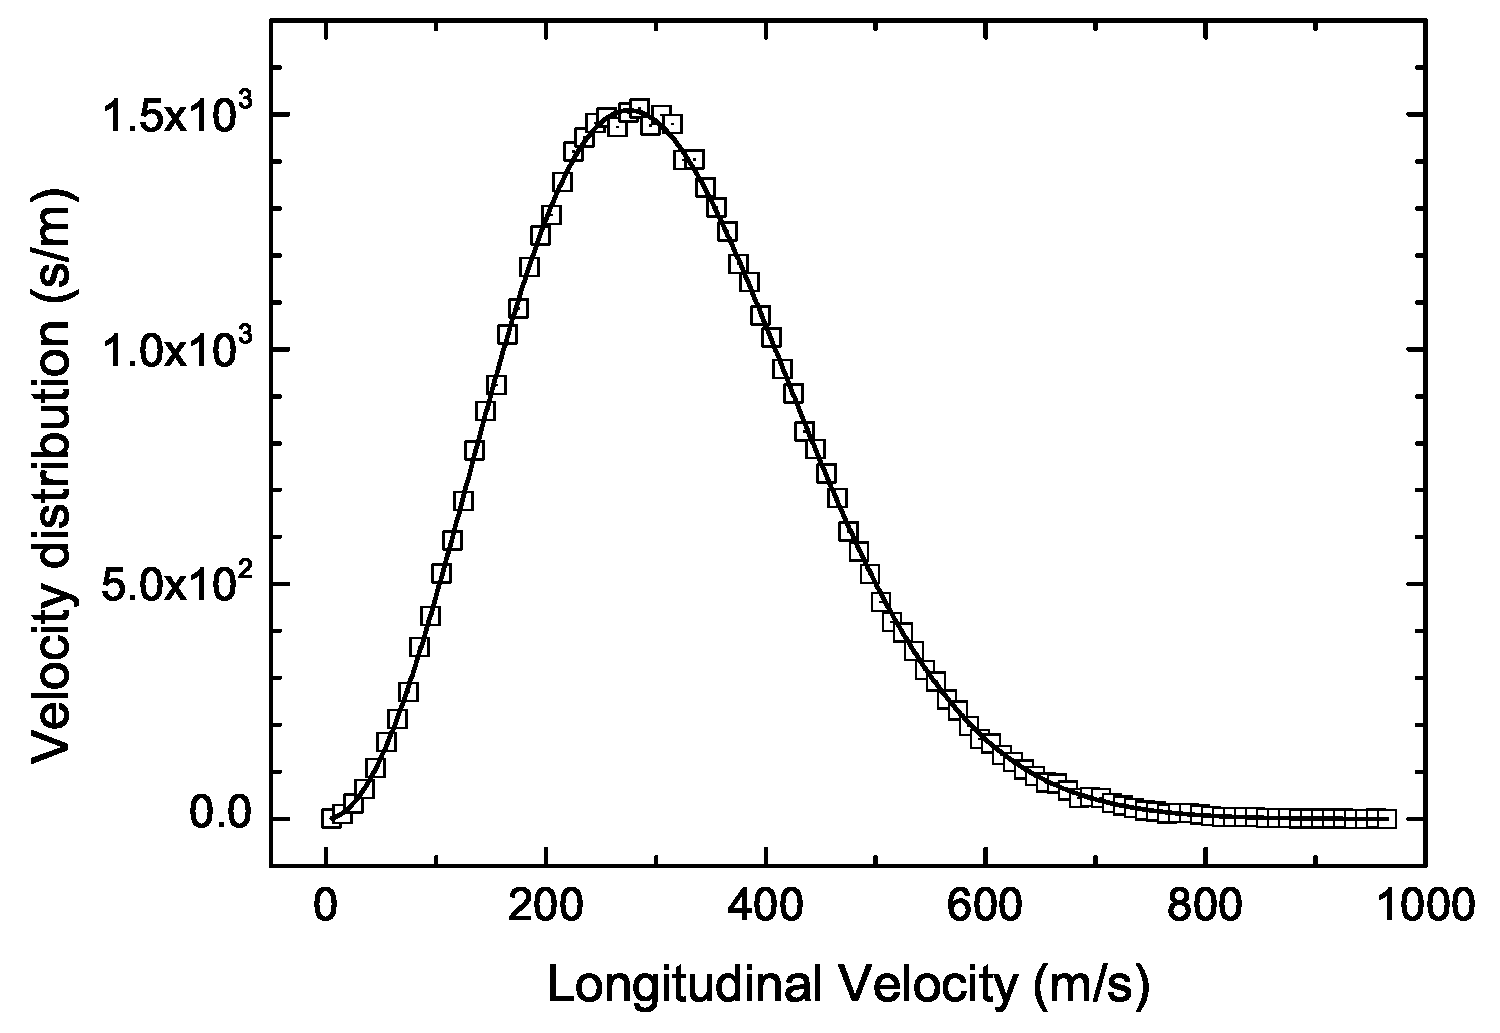
\includegraphics[width=0.7\linewidth]{pics/newsource/initVelocityDistrOptimized_Rb-87_500k_400K}
    \caption{Initial particle distribution of $N=5 \times 10^5$ $^{87}$Rb atoms at a temperature of 400 K. The distribution is normalized to $N$. The solid line is a fit of the normalized velocity distribution of equation (\ref{eq:initdistr_vel}).} 
    \label{fig:v_distr}
\end{figure}

After randomly picking an initial position $|x| \leq d$ on the aperture $A_i$, the angle $\alpha$ is then initialized. The angle $\alpha$ is also randomly picked according to the criteria
\begin{equation}
  	-\arctan\left({\frac{d-x}{l}}\right) \leq \alpha \leq \arctan\left({\frac{d+x}{l}}\right).
  	\label{eq:ang_criteria}
\end{equation}
The transverse velocity is then calculated as $v_x=\alpha~v_z$. This procedure is repeated for all the $N$ particles.
%The maximum angle is calculated as $\theta_{max} = 2 d/l$ and the number of particles per unit angle is given by
%\begin{equation}
%  	f_{ang}(\alpha) \rmd \alpha = C_0 (2 d-l~\tan(\alpha)) \rmd \alpha; \ \ \ \ \   0 \leq \alpha \leq \arctan(\theta_{max}),
%  	\label{eq:initdistr_ang}
%\end{equation}
%where $C_0$ is a normalization constant (proportional to the number of particles in the simulation). Similarly a particle distribution function can be derived for $\theta < 0$, and differs only by a minus sign from the previous formula. Since with our geometry $\alpha_{max} \ll 1$, it is possible to simplify the angular distribution as
%\begin{equation}
%  	f_{ang}(\alpha) \rmd \alpha \approx C_0 (2d \mp l~\alpha) \rmd \alpha; \ \ \ \ \   0 \leq |\alpha| \leq \theta_{max}.
%  	\label{eq:initdistr_ang2}
%\end{equation}


\subsection{Source characterization}
In this subsection, the definition of the current and the reduced brightness are given. Depending on the parameters, only a certain number of particles $N_f$ will make it through the final aperture $d_f$ and it is necessary to estimate at first the fraction of the flux that is carried by each particle.

The atomic flux $\Phi_i$ through the first aperture $A_i$ is given by
\begin{equation}
	\Phi_i = \frac{n}{4 \pi} \langle v \rangle \mathcal{F}(d,l),
	\label{eq:initflux}
\end{equation}
where in the case of $l \gg d$ \cite{Notermans2012}
\begin{equation}
%\mathcal{F}(d,l) = 8d \Bigg[ \sqrt{4 d^2 + l^2} \arctan \Bigg( \frac{2d}{\sqrt{4d^2+l^2}} \Bigg) - l \arctan \Bigg( \frac{2d}{l} \Bigg) \Bigg]
%+ 2l^2 \ln \Bigg( \frac{4d^2 + l^2}{\sqrt{8l^2d^2 + l^4}}  \Bigg).
	\mathcal{F}(d,l) = 16 \frac{d^4}{l^2} + o\left(\frac{d^6}{l^4}\right).
\label{eq:G_square}
\end{equation}
%A derivation of Eq. (\ref{eq:G_square}) is shown in the Appendix. 
The quantity $\mathcal{F}(d,l)=9.59 \times 10^{-11}$~m$^2$, using the values of $d$ and $l$ found in table \ref{tab:parametervalues_ana} (the result is valid for a square aperture and it differs only a factor $\pi/4$ from the one obtained with a circular aperture \cite{Notermans2012}). Equation (\ref{eq:initflux}) depends on geometrical variables: the free expansion length $l$ and the aperture size $d$, and on the source temperature $T_s$.

The final current $I(d_f)$ (of an ion beam with the same properties) depends on $d_f$ and it is calculated as
\begin{equation}
	I(d_f) = e~C \sum_{j=1}^{N_f(d_f)}{v_{z,j}^f},
	\label{eq:current_newsource}
\end{equation}
with $N_f$ as the number of particles passing through the final aperture $A_f$ and the normalization constant $C$ given by
\begin{equation}
	C = \frac{\Phi_i}{\sum_{j=1}^{N}{v_{z,j}^i}}.
	\label{eq:norma_flux}
\end{equation}
The quantities $v_{z,j}^i$ and $v_{z,j}^f$ respectively represent the initial longitudinal velocity (at the first aperture $A_i$) and the final longitudinal velocity (at the second aperture $A_f$) of the j-th particle.

The final reduced brightness $B_r(d_f)$ is then given by 
\begin{equation}
	B_r(d_f) = \frac{1}{4 \pi^2} \frac{I(d_f)}{\epsilon_r(d_f)},
	\label{eq:brightness}
\end{equation}
which can be derived from \cite{Luiten2007}. In equation (\ref{eq:brightness}), the reduced emittance $\epsilon_r$ of the beam at a fixed position $z$ is given by \cite{Floettmann2003}
\begin{equation}
	\epsilon_r(d_f) = \epsilon_r^x(d_f) \epsilon_r^y(d_f) \approx [\epsilon_r^x(d_f)]^2 = \frac{m}{2} \left[ \left\langle x^2 \right\rangle \left\langle v_x^2 \right\rangle - \left\langle x~v_x \right\rangle^2 \right],
	\label{eq:emittance}
\end{equation}
where $\langle \rangle$ defines the average over the particle ensemble. In equation (\ref{eq:emittance}), since the two orthogonal directions are independent due to the square geometry, the approximation $\epsilon_r^x \approx \epsilon_r^y$ is used.\\
Figure \ref{fig:BrandI_VSaperture_Rb87} shows the reduced brightness plotted versus the final aperture size $d_f$ in case of $^{87}$Rb, using the parameters shown in table \ref{tab:parametervalues}. 
\begin{equation}
	B_r^p = \frac{1}{4 \pi^2} \frac{I^p}{\epsilon_r^p},
	\label{eq:brightness10}
\end{equation}
where the superscript $p$ denotes that only the 10\% of the particles closest to the \textit{z}-axis are used and $I^p=I/10$. The brightness calculated with equation (\ref{eq:brightness10}) approximates the value for $d_f \to 0$ (which can not be calculated numerically) and from now on it will be named peak brightness.\\
Figure \ref{fig:BrandI_VSaperture_Rb87} also shows the current versus the final aperture size and it can be seen that an aperture size $d_f=1~\mu$m corresponds to about $I=30$~pA. The plot also shows that the current density is constant up to $d_f=5~\mu$m, where a current on the order of 1~nA can be achieved.
\begin{figure}[tbh!]
    \centering
        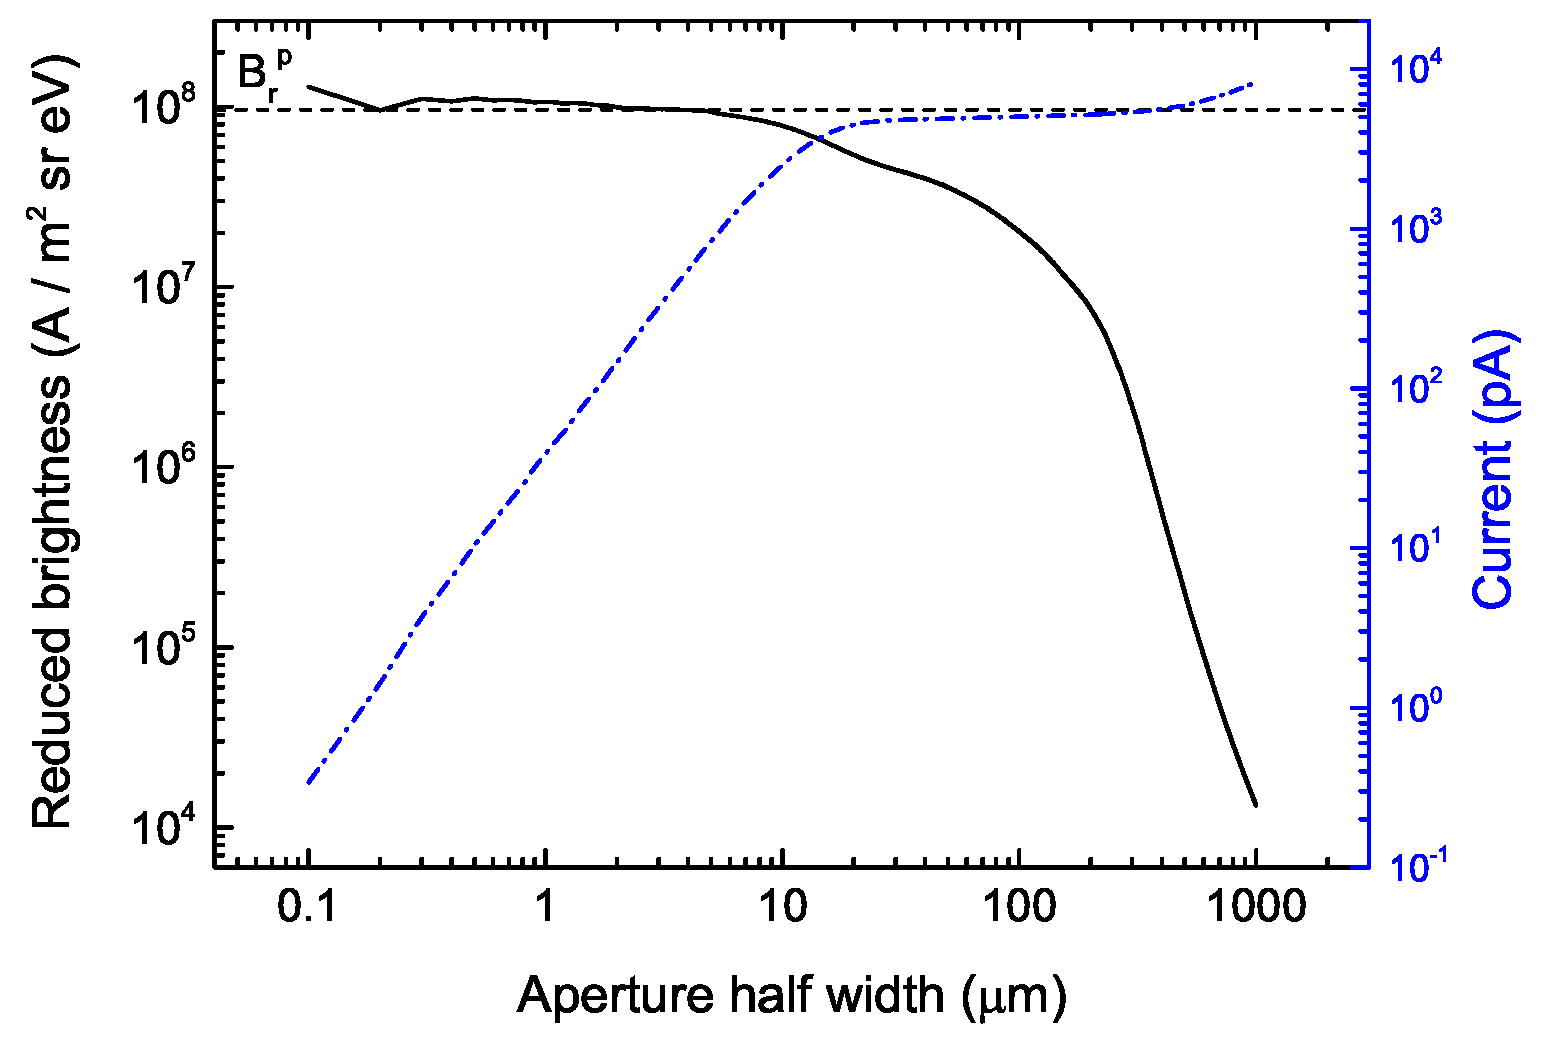
\includegraphics[width=0.7\linewidth]{pics/newsource/BrandI_VSaperture_Rb87}
    \caption{The reduced brightness $B_r$ at the end of the MOC plotted versus the final aperture size $d_f$ (solid line) on a double logarithmic scale. The dashed line indicates the reduced peak brightness $B_r^p$ as defined in equation (\ref{eq:brightness10}). Also, the current is plotted as a dash-dot line. Both of the curves are obtained with $^{87}$Rb, see table \ref{tab:parametervalues}.} 
    \label{fig:BrandI_VSaperture_Rb87}
\end{figure}

Figure \ref{fig:initdistrGPT} shows a plot of the particle distribution (same data set of figures \ref{fig:v_distr} and \ref{fig:BrandI_VSaperture_Rb87}) at the end of the MOC for $N=1.4 \times 10^5$ $^{87}$Rb atoms. The plot is binned and the color code represents the areal particle density but since the plot is intended for qualitative purpose, no color scale is added. The \textit{rms}-size of the full ensemble is $\sigma_x^{rms} = 258~\mu$m and the \textit{rms}-size of the 10\% of the particles closest to the $z$-axis is $\sigma_x^p = 2.9~\mu$m. In the $y$-direction, the sizes are approximately the same. From this plot, it is clear that the final aperture $A_f$ is necessary in order to skim off the low-brightness tails that are apparent as wings to the distribution. An aperture with a half width $d_f=30~\mu$m contains 95\% of the particles shown in the figure (the aperture is drawn in the figure as a solid square).
\begin{figure}[tbh!]
    \centering
        \includegraphics[width=0.6\linewidth]{pics/newsource/initdistrGPT}
    \caption{Particle spatial distribution at the end of the MOC for $N=1.4 \times 10^5$ $^{87}$Rb atoms. The plot is binned and the color code represents the areal particle density, ranging from blue (low density) to yellow (high density). The plot is shown for qualitative purpose and no color scale is shown. The \textit{rms}-size of the full ensemble is $\sigma_x^{rms} \approx \sigma_y^{rms} = 258~\mu$m and $\sigma_x^p \approx \sigma_y^p = 2.9~\mu$m, considering only the 10\% of the particles closest to the \textit{z}-axis. The 95\% of the particles shown in the figure is contained within an aperture half width $d_f=30~\mu$m, indicated in the figure as a solid square.} 
    \label{fig:initdistrGPT}
\end{figure}

Figure \ref{fig:initdistrGPT_phsp} shows the $(x-v_x)$ phase-space plot of the particle distribution at the end of the MOC. 
\begin{figure}[tbh!]
    \centering
        \includegraphics[width=0.6\linewidth]{pics/newsource/initdistrGPT_phsp}
    \caption{Particle $(x-v_x)$ phase-space distribution at the end of the MOC for $N=1.4 \times 10^5$ $^{87}$Rb atoms. The plot is binned and the color code represents the areal particle density, ranging from blue (low density) to yellow (high density). The plot is shown for qualitative purpose and no color scale is shown. The picture in the insert is a larger view from in the horizontal scale, from -1~mm  to 1~mm.} 
    \label{fig:initdistrGPT_phsp}
\end{figure}
In this figure, we can see that there is a central ``core'' of particles close to the axis that have been cooled and compressed. Around this core, we note the presence of many particles that have not been compressed or not been cooled sufficiently; those particles tend to be correlated in $(x-v_x)$ phase-space, meaning that a particle further away from the origin, most likely has a larger transversal velocity. The inserted box shows a larger view of the same figure. %but the ``s'' shape in the phase-space does not lead to a simple explanation. 

\section{Results and comparison}\label{sec:results}
In this section, the analytical model is used as a benchmark to compare the performance of the simulations. Table \ref{tab:parametervalues_ana} shows the parameters used for the comparison in case of an ideal 2-level $^{85}$Rb atom, used both for the model and the simulation. Once the comparison is made, this set of parameter is used as a starting point for the simulations. With the simulations, each of the parameters is optimized individually, at first also for a 2-level $^{85}$Rb atom and later on for realistic $^{85}$Rb and $^{87}$Rb atoms. Table \ref{tab:parametervalues} summarizes the values used for simulation of the best case scenario in case of realistic rubidium (rubidium with its real level scheme instead of the ideal 2-level system). The dependence of the simulations on $d$ and $l$ is not shown in this paper in order to reduce the number of variables and the values of these geometrical quantities are kept constant for the simulations shown here (see table \ref{tab:parametervalues_ana}). A few examples of the atomic beams with the best brightness are used as initial particle distribution in GPT. With GPT the atomic beam is ionized and the effect of the disorder-induced heating on the ion beam is included.

\begin{table}[h!]
	\centering
	\caption{Parameter values for the simulation with $^{85}$Rb and $^{87}$Rb. The values of $d=3.1~\times~10^{-4}$~m and $l=3.9~\times~10^{-2}$ are used, as it is already shown in table \ref{tab:parametervalues_ana}.}
	\begin{center}
		\begin{tabular}{|l|l|l|l|} \hline
		{Parameter (unit)} & {Symbol} & {$^{85}$Rb} & {$^{87}$Rb}	\\ \hline
		{Source temperature (K)} & $T_s$ & {$400$} & {$400$}	\\ 
		{Cooling and compression length (m)} & $L$ & {$0.1$} & {$0.1$}	\\ 
		{Saturation parameter (-)} & $s_0$ & {$1.5$} & {$1.5$}	\\ 
		{Detuning ($\Gamma$)} & $\delta$ & {$-0.5$} & {$-0.6$}	\\
		{Magnetic gradient (T/m)} & $G$ & {$4$} & {$2.5$}	\\ \hline
		\end{tabular}
	\end{center}
	\label{tab:parametervalues}
\end{table}

\subsection{Comparison of the analytical model with the simulations}
The analytical model, discussed in section \ref{sec:anamodel}, assumes that all the 2-level $^{85}$Rb atoms passing through the first aperture $A_i$, are cooled and compressed down to the final aperture $A_f$, where they have reached equilibrium. The simulations are performed also with a 2-level $^{85}$Rb atom and show for which compression length this assumption is valid. The values of the parameters used for this comparison are shown in table \ref{tab:parametervalues_ana}. For this comparison, the theoretical Doppler temperature $T_D$ in the model is replaced with the one calculated from the simulations output $T_f=\sigma_v^2 m/k_b$, with the quantity $\sigma_v$ as the \textit{rms}-transverse velocity. Figure \ref{fig:comp_temp} shows a comparison between simulations obtained varying the source temperature at different lengths, $L=0.05,\: 0.1,\: 0.2, \: 1$ m (scattered). The solid line is the result of the analytical model.
\begin{figure}[tbh!]
    \centering
        \includegraphics[width=0.7\linewidth]{pics/newsource/BrVS_Ts_L}
    \caption{Reduced peak brightness $B_r^p$ plotted on a logarithmic scale as a function of the source temperature $T_s$, for different cooling and compression stage lengths $L$. As $L$ increases, the beam is cooled and compressed more into equilibrium and the simulation results (scattered) converge to the analytical results (solid line). A 2-level $^{85}$Rb atom is used in those simulations and calculation. The used parameters are given in table \ref{tab:parametervalues_ana}.} 
    \label{fig:comp_temp}
\end{figure}
A higher source temperature means, on the one hand, a higher initial flux, but on the other hand, since the longitudinal velocity increases, an atom spends less time in the MOC section, so that the brightness increases less rapidly for a higher source temperature. For a short compression length, the simulation result differs more than an order of magnitude from the result of the analytical model. At $L=1$ m, the simulation data (scattered in red) converge to the analytical result (solid line), as expected. From this plot, it can be seen that it is convenient to increase the length $L$ from 5~cm to 10~cm, gaining a factor $(6.1~\pm~0.5)$ in the reduced brightness.\\

By varying the detuning, the damping and spring constants can be varied. With a lower detuning, the force becomes stronger but the capture range decreases. Generally, the most effective cooling and compression is reached at $\delta=-\Gamma/2$. Figure \ref{fig:comp_detu} shows the reduced brightness versus the detuning simulated at different compression lengths. The maximum achievable brightness is, as expected, near a detuning of $\delta =	-\Gamma/2$, but generally a long interaction length is required for the beam to reach equilibrium and to converge to the analytical result. A value $\delta = -\Gamma/2$ works best for both model and simulations.
\begin{figure}[tbh!]
    \centering
        \includegraphics[width=0.7\linewidth]{pics/newsource/BrVSdetu_L}
    \caption{Reduced peak brightness $B_r^p$ plotted on a logarithmic scale as a function of the detuning, for different cooling and compression stage lengths $L$. As $L$ increases, the beam is cooled and compressed more into equilibrium and the simulation results (scattered) converge to the analytical results (solid line). A 2-level $^{85}$Rb atom is used in those simulations and calculation. The parameters used are given in table \ref{tab:parametervalues_ana}.} 
    \label{fig:comp_detu}
\end{figure}

\subsection{Parameter optimizations for a 2-level $^{85}$Rb atom}
Several simulations, in which only one parameter at a time is varied, are performed in order to optimize the reduced peak brightness in the parameter phase-space. Those simulations run for a range of values of a second parameter. Figure \ref{fig:BrVSdetu_grad} shows a plot of the reduced peak brightness versus the detuning for three different magnetic field gradient values. Figure \ref{fig:BrVSgrad_detu}, instead, at four different detuning values, plots the reduced brightness versus the magnetic field gradient. Those figures show that we need a sufficiently large gradient to force atoms to the axis in the given length, but if the gradient is too high, the brightness is decreased because the capture radius becomes smaller than the aperture size $d$. This is in contrast with the analytical model, where the brightness linearly depends on the magnetic gradient field.
\begin{figure}[tbh!]
    \centering
        \includegraphics[width=0.7\linewidth]{pics/newsource/BrVSdetu_grad}
    \caption{Reduced peak brightness $B_r^p$ as a function of the detuning $\delta$ for different magnetic field gradients $G$ and for a 2-level $^{85}$Rb atom. The optimum of brightness is attained at $\delta = - 0.6~\Gamma$ and for $G=1$ T/m. All other simulation parameters are given in table \ref{tab:parametervalues_ana}.} 
    \label{fig:BrVSdetu_grad}
\end{figure}
\begin{figure}[tbh!]
    \centering
        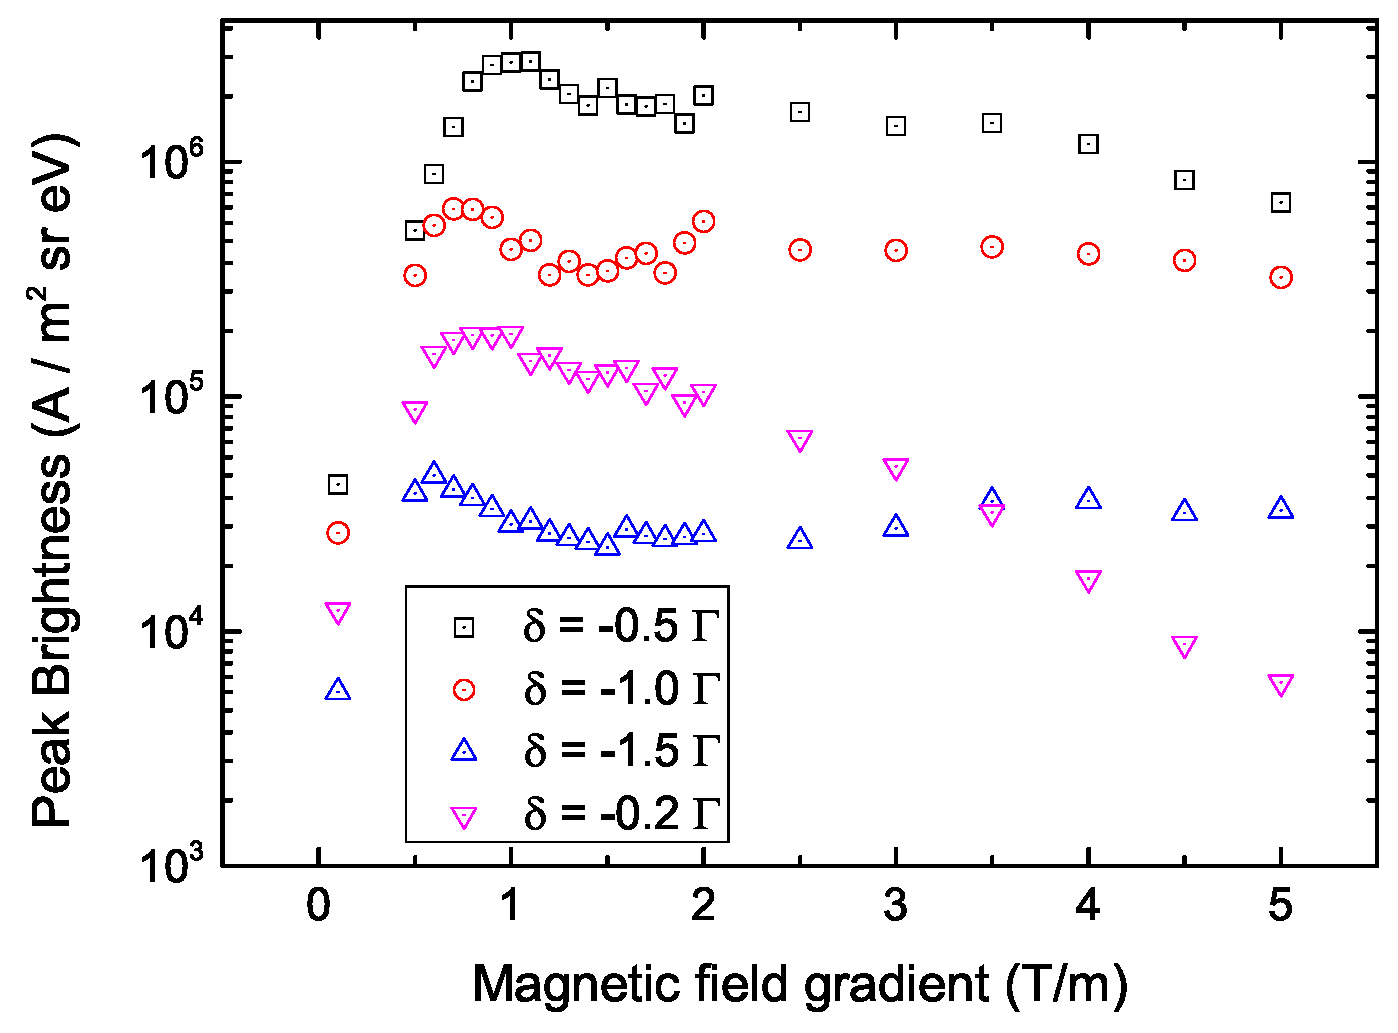
\includegraphics[width=0.7\linewidth]{pics/newsource/BrVSgrad_detu}
    \caption{Reduced peak brightness $B_r^p$ as a function of the magnetic field gradients $G$ for different detunings $\delta$ and for a 2-level $^{85}$Rb atom. The optimum of brightness is attained at $G=1$ T/m and for $\delta = - \Gamma/2$. All other simulation parameters are given in table \ref{tab:parametervalues_ana}.} 
    \label{fig:BrVSgrad_detu}
\end{figure}
With this ``double check'' technique, it is possible to maximize the reduced peak brightness for two parameters at the same time. In this case, it confirms that the highest brightness for a 2-level $^{85}$Rb atom is attained for values close to the ones shown in table \ref{tab:parametervalues_ana}: at $G = 1$ T/m and $\delta = -0.6~\Gamma$. In table \ref{tab:parametervalues_ana} also the other parameters used for this section are summarized.

\subsection{Realistic rubidium atom results}
All the aforementioned analysis has been performed for an ideal 2-level $^{85}$Rb atom. As a real rubidium atom has a more complicated level structure, the cooling and compression will be less efficient. Hence it is expected that using real rubidium will result in a lower brightness compared to the 2-level $^{85}$Rb case. The atomic $^{85}$Rb and $^{87}$Rb properties are shown in table \ref{tab:Rb_atomic_consts}. Furthermore, the parameters of the real rubidium atom will need to be optimized differently. Nevertheless, the parameter values shown in table \ref{tab:parametervalues_ana} are a good starting point for this procedure. In particular, we find that $^{85}$Rb requires a larger field gradient than $^{87}$Rb, which in turn requires a larger field gradient than a 2-level $^{85}$Rb atom.

A comparison of the 2-level $^{85}$Rb with $^{85}$Rb and $^{87}$Rb is shown in Figure \ref{fig:BrVS_L_elements}.
\begin{figure}[tbh!]
    \centering
        \includegraphics[width=0.7\linewidth]{pics/newsource/BrVS_L_elements}
    \caption{Reduced peak brightness $B_r^p$ plotted as a function of the cooling and compression stage length $L$ on a logarithmic scale, for 2-level $^{85}$Rb, $^{85}$Rb and $^{87}$Rb. Due to a more complicated level structure of the realistic atoms, the laser cooling and compression is less efficient, resulting in a lower brightness. The $^{87}$Rb performs better than $^{85}$Rb, since $^{87}$Rb has a lower nuclear spin (respectively 3/2  versus 5/2), which results in a larger transition strength when averaged over all ground-state sub-levels. In these simulation, the parameters from tables \ref{tab:parametervalues_ana} and \ref{tab:parametervalues} are used.} 
    \label{fig:BrVS_L_elements}
\end{figure}
From this plot, it can be seen that the $^{87}$Rb isotope performs better than $^{85}$Rb, as the $^{87}$Rb atom has a lower nuclear spin quantum number than $^{85}$Rb (respectively 3/2  versus 5/2) which results in a larger transition strength when averaged over all ground-state sub-levels. Hence it is advisable to use $^{87}$Rb to improve the performance of the source. The abundance of the isotopes is not taken into account in the definition of reduced brightness but even when taking it into account, $^{87}$Rb would still reach a reduced brightness about 1.6 times larger than $^{85}$Rb.\\
Moreover, from this plot it is possible to fix the value of $L$ as discussed already for figure \ref{fig:comp_temp}. The brightness increases a factor of 6.5 going from 5 cm to 10 cm (for $^{87}$Rb). In case of $L=20$ cm, this increase in brightness is less pronounced (a gain of 2.5). The choice $L=10$~cm still keeps the setup compact. It looks like the $^{85}$Rb isotope requires a longer length than the $^{87}$Rb one, which makes sense due to the higher nuclear spin quantum number of the latter isotope.

Figure \ref{fig:BrVS_I_elements} summarizes the optimized performance of the atomic source for a range of source parameters, and shows that using a realistic rubidium isotope, peak brightnesses in the range of $10^7 - 10^8$ A / m$^2$ sr eV can be achieved with currents of $100 - 1000$ pA. In these simulation the parameters from tables \ref{tab:parametervalues_ana} and \ref{tab:parametervalues} are used.
\begin{figure}[tbh!]
    \centering
        \includegraphics[width=0.7\linewidth]{pics/newsource/BrVS_I_elements}
    \caption{Reduced peak brightness $B_r^p$ as function of the peak current for 2-level $^{85}$Rb, $^{85}$Rb and $^{87}$Rb. This is simulated at different source temperatures. The dotted and the solid circles group together the measurements performed at the same source temperature. The solid circle evidences the chosen temperature of 400 K. Due to a more complicated level structure of the real atoms, the laser cooling and compression is less efficient, resulting in a lower brightness for equal currents. In these simulation the parameters from tables \ref{tab:parametervalues_ana} and \ref{tab:parametervalues} are used.} 
    \label{fig:BrVS_I_elements}
\end{figure}
Again, $T_s=400$~K seems a good choice since at at this temperature the mean free path of the particles is still larger than the size of the hole in the Knudsen cell.

A summary of the optimization for $^{85}$Rb and for $^{87}$Rb is shown in table \ref{tab:parametervalues}. Those results, however, are an upper limit for the brightness of the ion beam that will be produced from the atomic beam, as disorder-induced heating is not taken into account yet (see section \ref{sec:GPTresults}).


\subsection{Disorder-induced heating effect on the ion beam} \label{sec:GPTresults}
To study the effect of disorder-induced heating on the ion beam, we feed the particle distribution obtained from the laser cooling simulations into GPT. %The 1-dimensional results of COOL are combined to the 2-dimensional case. 
GPT generates particles according to the rate given by the flux of atoms simulated with COOL, and with a temporal, spatial and velocity distribution corresponding to that at the end of the compressor stage (also from COOL). The atomic beam is tracked depending on a final aperture size $d_f$. The atomic beam then passes through an ionization region with a \textit{rms}-radius $\sigma_i = 1~\mu$m, so that ions are created along the z-direction with a quasi-Gaussian shape (the ionization fraction is set to one, which is realistic for a high power CW laser beam). This value is chosen since it is feasible (not easily achievable) to focus a 480~nm laser beam to a size $\sigma_i = 1~\mu$m (attainable with a lens with 0.4 numerical aperture, as the LMH-20X-532 from Thor Labs \cite{thorlabs}). The ions are accelerated with a homogeneous electric field $\vec{E}$ and travel toward a screen at a distance of 0.1~m. GPT solves the equations of motion and takes into account all the mutual Coulomb interactions between ions \cite{gpt}. With an aperture in the order of a few $\mu$m size, the so-called pencil-beam regime \cite{Tiemeijer1999} can be reached. In this regime, there is no transverse heating and hence no reduction in brightness because the spacing between particles is larger than the beam size, i.e. ions have no neighbor in the transverse direction.

Figure \ref{fig:GPT_result} plots the reduced brightness versus the current (which is controlled by varying the aperture size $d_f$). The ion beam corresponds to the best cooling result obtained from the simulation of a $^{87}$Rb atomic beam using the parameters summarized in table \ref{tab:parametervalues}.
\begin{figure}[tbh!]
    \centering
        \includegraphics[width=0.7\linewidth]{pics/newsource/GPTresult}
    \caption{Reduced brightness plotted versus the extracted current on a double logarithmic scale. The curves are calculated with GPT. The dashed line is in case of no space charge forces taken into account (SC off). The solid lines are in presence of space charge forces. The black solid line is for an extraction field of 2.5~MV/m which results in an energy spread of 3.3~eV. The red solid line is for an extraction field of 0.5~MV/m which results in an energy spread of 0.7~eV.} 
    \label{fig:GPT_result}
\end{figure}
The figure plots the case with space charge forces not taken into account (dashed line) and two examples of beams with a different energy spread (solid lines). With energy spread we mean the 50\% energy spread. The difference in energy spread is a consequence of the different electric field used to accelerate the ions. The figure shows that disorder-induced heating has a very large influence and quickly decreases beam brightness for increasing current. However, for currents up to 10s of pA (depending on the extraction electric field), the reduced brightness is preserved because of the pencil-beam regime. In this regime, the simulations with GPT show that at an impressive reduced brightness of $2 \times 10^7$~A/m$^2$~sr~eV and an ion current of 22~pA can be simultanously achieved. This current is obtained using an aperture $d_f = 1.6~\mu$m which is given by 
\begin{equation}
	d_f~{\rm(\mu m)} =2 \times 10^{-0.78} \sqrt{I~\rm{(pA)}}. 
	\label{eq:f_diameter}
\end{equation}
Current and aperture size follow a linear relationship in the current range 1-1000 pA used in GPT simulations.
The energy spread is 0.7~eV, resulting from an extraction electric field of 0.5~MV/m. Under these conditions, this source performs substantially better than the LMIS, reaching a 6.4 times lower energy spread with a 20 times better reduced brightness and the extracted current is large enough for FIB applications. Those results are achieved with a $^{87}$Rb isotope used in the Knudsen cell. Using $^{85}$Rb would result in about 4 times lower brightness with respect to $^{87}$Rb. As mentioned before, we assume that purified sources are used. 
With an extraction field of 2.5~MV/m, corresponding to an energy spread of 3.3~eV, a beam current of 300~pA at a reduced brightness of $10^6$~A/m$^2$~sr~eV can be achieved. This current is obtained using a final aperture size $d_f=5.7~\mu$m, from equation (\ref{eq:f_diameter}). Those values of reduced brightness and energy spread are comparable to the ones of the LMIS.

\section{Conclusion and discussion}
%- present case of Litium and an heavy metal to compare.

In this paper we explore whether the ABLIS could improve the current state of art of ion sources for FIBs. We demonstrate with simulations the high potential of this source in terms of brightness and energy spread. The strength of the source is in its compactness and high atomic flux effusing from a Knudsen cell. For instance at a source temperature $T_s=400$~K a flux $\Phi_i=3 \times 10^{10}$ particles per second goes through the first aperture $A_i$ (for the geometry considered in this paper), which would correspond to an atomic current of 4.7~nA. With laser cooling and compression, this flux gives rise to a high-brightness atomic beam that can be turned into an ion beam using photo-ionization.

Before performing the simulations, we have attempted to analytically model the behavior of the source. This modeling is used to optimize the reduced peak brightness of an unrealistic, but very useful, 2-level $^{85}$Rb atom. The conclusions of the model are used as a starting point for the simulations. The analytical brightness depends on geometrical variables (the expansion length $l$, the aperture $d$ and the compression length $L$), on laser cooling variables (detuning $\delta$ and saturation parameter $s_0$), on the magnetic gradient $G$ used to compress the beam, and finally on the source temperature of the Knudsen cell $T_s$. The dependences on $d$ and $l$ are not shown in this paper and the values estimated with the analytical model are kept constant in the simulations. With the model it is possible to optimize the laser parameters, while the geometry and the magnetic gradient are fixed in order to keep the setup small and to reproduce realistic achievable fields. The source temperature is set so that the mean free path of the particles is much larger than the opening of the Knudsen cell.

The simulations are performed with realistic rubidium. The $^{87}$Rb isotope is found to reach higher atomic beam reduced brightnesses due to its lower nuclear spin with respect to the $^{85}$Rb isotope, which results in a larger transition strength when averaged over all ground-state sub-levels. The upper limit of the reduced peak brightness equals $10^8$~A/m$^2$~sr~eV in the best case scenario. Taking into account disorder-induced heating, reduces the ionic beam reduced peak brightness by 2-3 orders of magnitude depending on the aperture size $A_f$. But in certain conditions, the so-called pencil-beam regime is reached and the disorder-induced heating does not deteriorate the brightness anymore. In this regime, a reduced brightness of $2 \times 10^7$~A/m$^2$~sr~eV with an ion current of 22 pA ($d_f=1.6~\mu$m) and an energy spread of 0.7 eV can be achieved. This is obtained with a $^{87}$Rb$^+$ beam originating from a purified source. In case of using natural abundance material, the brightness must be corrected with the abundance of the isotope (about one quarter).

Obviously there will be many technical challenges in constructing such a source. For instance, large-diameter laser beams with (preferably) extreme aspect ratio are required, for which suitable optical elements are not readily available. The intensity balance between the beams, their separate temporal and spatial intensity stability could be an issue, as well as local variations of the magnetic field. In addition, near the end of the compressor stage the atomic beam may become optically thick, at which point laser cooling becomes less effective. This regime is in fact approached for an atomic beam carrying the equivalent of 1~nA of current in a 10~$\mu$m diameter traveling at a few 100 m/s. Further investigation of these issues through simulations and experimentation may be required to realize such a source.

\clearpage

\bibliographystyle{unsrt}

\begin{thebibliography}{10}

\bibitem{Orloff_RoSI_93}
J.~Orloff.
\newblock {H}igh-resolution focused ion beams.
\newblock {\em Rev. Sci. Instrum.}, 64(5):1105--1130, 1993.

\bibitem{Moore_E_65}
G.E. Moore.
\newblock {C}ramming more components onto integrated circuits.
\newblock {\em Electronics}, 38/8, 1965.

\bibitem{Debernardi2012}
N.~Debernardi, R.W.L. Vliembergen, W.~J. Engelen, K.H.M. Hermans, M.P.
  Reijnders, S.~van~der Geer, P.~H.~A. Mutsaers, O.~J. Luiten, and E.~J.~D.
  Vredenbregt.
\newblock {O}ptimization of the current extracted from an ultracold ion source.
\newblock {\em New J. Phys.}, SUBMITTED.

\bibitem{Reijnders_PRL_09}
M.~P. Reijnders, P.~A. van Kruisbergen, G.~Taban, S.~B. van~der Geer, P.~H.~A.
  Mutsaers, E.~J.~D. Vredenbregt, and O.~J. Luiten.
\newblock {L}ow-{E}nergy-{S}pread {I}on {B}unches from a {T}rapped {A}tomic
  {G}as.
\newblock {\em Phys. Rev. Lett.}, 102(3):034802, 2009.

\bibitem{Hanssen_PRA_06}
J.~L. Hanssen, J.~J. McClelland, E.~A. Dakin, and M.~Jacka.
\newblock {L}aser-cooled atoms as a focused ion-beam source.
\newblock {\em Phys. Rev. A: At. Mol. Opt. Phys.}, 74(6):063416, 2006.

\bibitem{Hanssen_NL_08}
J.~L. Hanssen, S.~B. Hill, J.~Orloff, and J.~J. McClelland.
\newblock {M}agneto-{O}ptical-{T}rap-{B}ased, {H}igh {B}rightness {I}on
  {S}ource for {U}se as a {N}anoscale {P}robe.
\newblock {\em Nano Lett.}, 8(9):2844--2850, 2008.

\bibitem{Steele_JVSTB_10}
A.~V. Steele, B.~Knuffman, J.~J. McClelland, and J.~Orloff.
\newblock {F}ocused chromium ion beam.
\newblock {\em J Vac Sci Technol B}, 28(6):C6F1--C6F5, 2010.

\bibitem{Freinkman2004}
B.G. Freinkman, A.V. Eletskii, and S.I. Zaitsev.
\newblock A proposed laser source of ions for nanotechnology.
\newblock {\em Microelectronic Engineering}, 73-74(0):139 -- 143, 2004.

\bibitem{Tempelaars2002}
J.G.C Tempelaars, R.J.W. Stas, P.G.M. Sebel, H.C.W. Beijerinck, and E.J.D.
  Vredenbregt.
\newblock An intense, slow and cold beam of metastable ne(3s) 3p2 atoms.
\newblock {\em Eur. Phys. J. D}, 18(1):113--121, 2002.

\bibitem{Lison1999}
F.~Lison, P.~Schuh, D.~Haubrich, and D.~Meschede.
\newblock High-brilliance zeeman-slowed cesium atomic beam.
\newblock {\em Phys. Rev. A}, 61:013405, 1999.

\bibitem{Tiemeijer1999}
P.C. Tiemeijer.
\newblock Measurement of coulomb interactions in an electron beam
  monochromator.
\newblock {\em Ultramicroscopy}, 78(1-4):53--62, 1999.

\bibitem{Vredenbregt_AJoP_03}
E.~J.~D. Vredenbregt and K.~A.~H. van Leeuwen.
\newblock {L}aser cooling and trapping visualized.
\newblock {\em American Journal of Physics}, 71(8):760--765, 2003.

\bibitem{Metcalf_Book_99}
H.J. Metcalf and P.~van~der Straten.
\newblock {\em {L}aser {C}ooling and {T}rapping}.
\newblock Springer, 1999.

\bibitem{gpt}
http://www.pulsar.nl/gpt.

\bibitem{Haynes_Book_12}
W.~M. Haynes, editor.
\newblock {\em {H}andbook of {C}hemistry and {P}hysics}.
\newblock "Vapor Pressure of the Metallic Elements" by C. B. Alcock,. CRC
  Press/Taylor and Francis, Boca Raton, FL, 92th edition, 2012.

\bibitem{Haynes_Book_12_b}
W.~M. Haynes, editor.
\newblock {\em {H}andbook of {C}hemistry and {P}hysics}.
\newblock "Table of the Isotopes" by N.E. Holden. CRC Press/Taylor and Francis,
  Boca Raton, FL, 92th edition, 2012.

\bibitem{Luiten_IJoMPA_07}
O.~J. Luiten, B.~J. Claessens, S.~B. van~der Geer, M.~P. Reijnders, G.~Taban,
  and E.~J.~D. Vredenbregt.
\newblock {U}ltracold {E}lectron {S}ources.
\newblock {\em Int. J. Mod. Phys. A}, 22/22:3882--3897, 2007.

\bibitem{Foot_Book_05}
C.~J. Foot.
\newblock {\em {A}tomic {P}hysics}.
\newblock Oxford University Press, 2005.

\bibitem{Blundell_Book_06}
S.J. Blundell and K.~M. Blundell.
\newblock {\em {C}oncepts in {T}hermal {P}hysics}.
\newblock Oxford University Press, 2006.

\bibitem{Mantina2009}
M.~Mantina, A.~C. Chamberlin, R.~Valero, R.~J. Cramer, and D.~G. Truhlar.
\newblock Consistent van der waals radii for the whole main group.
\newblock {\em J. Phys. Chem. A}, 113:5806--5812, 2009.

\bibitem{Scoles1988}
G.~Scoles.
\newblock {\em {A}tomic and molecular beam methods, Volume 1}.
\newblock Oxford University Press, 1988.

\bibitem{Notermans2012}
R.P.M.J.W. Notermans.
\newblock Master's thesis, Eindhoven University of Technology, 2012.

\bibitem{Luiten2007}
O.~J. Luiten, B.~J. Claessens, S.~B. van~der Geer, M.~P. Reijnders, G.~Taban,
  and E.~J.~D. Vredenbregt.
\newblock Proceedings of the 46th workshop of the infn eloisatron project.
\newblock In {\em The physics and applications of high brightness electron
  beams}. World Scientific Publishing Co. Pte. Ltd., 2007.

\bibitem{Floettmann2003}
K.~Floettmann.
\newblock Some basic features of the beam emittance.
\newblock {\em Phys. Rev. ST Accel. Beams}, 6:034202, 2003.

\bibitem{thorlabs}
www.thorlabs.com.

\end{thebibliography}


%\end{document}